\documentclass[11pt,reqno]{amsart}
\usepackage{graphicx}
\usepackage{enumerate}
\usepackage{mathtools}
\usepackage[margin=1in]{geometry}
\usepackage{booktabs}
\usepackage{graphicx}
\usepackage{amsmath}
\usepackage{hyperref}
\usepackage{subcaption} % 导入 subcaption 包以支持子图
\usepackage{float}
\renewcommand{\theequation}{\arabic{enumi}.\arabic{equation}}

\DeclareMathOperator{\im}{im}
\DeclareMathOperator{\rank}{rank}
\DeclareMathOperator{\nullity}{nullity}
\DeclareMathOperator{\tr}{tr}

\newcommand{\tp}{{\scriptscriptstyle\mathsf{T}}}
\usepackage{listings} 
\usepackage{xcolor} 
\lstset{
  language=C++,                 % 设置语言为 C++
  basicstyle=\ttfamily,          % 使用等宽字体
  keywordstyle=\color{blue},     % 关键字高亮为蓝色
  commentstyle=\color{green},    % 注释高亮为绿色
  stringstyle=\color{red},       % 字符串高亮为红色
  numberstyle=\tiny\color{gray}, % 行号高亮为灰色
  numbers=left,                  % 行号显示在左侧
  stepnumber=1,                  % 每行显示行号
  frame=single,                  % 给代码加一个边框
  breaklines=true,               % 自动换行
  backgroundcolor=\color{lightgray!20}, % 设置背景颜色
  captionpos=b,                  % 标题在底部
  showspaces=false,              % 显示空格
  showstringspaces=false,        % 在字符串中显示空格
}
\lstdefinestyle{python}{
    language=Python,
    basicstyle=\ttfamily\small,  % Code font size
    keywordstyle=\bfseries\color{blue},
    commentstyle=\itshape\color{green!50!black},
    stringstyle=\color{orange},
    showstringspaces=false,
    frame=single,                % Adds a border around the code
    numbers=left,                % Line numbers on the left
    numberstyle=\tiny\color{gray},
    breaklines=true,             % Automatic line breaking
    captionpos=b,                % Caption at the bottom
    tabsize=4,                   % Tab size
}
\setlength{\parindent}{0pt}
\begin{document}
\title[]{Project1:Inverse problems with ML surrogate models\\Chu Zhuyiheng 12455799}
\maketitle


\section{Solve an inverse problem in the numerical Lorenz96 model}

The script \verb|mcmc_num.py| has completed the task, where the adjustable parameter is \verb|num_samples|, which specifies the number of samples drawn using the MCMC method. I used the latter half of the samples as output values for subsequent analysis, while discarding the first half as the burn-in period.

x0 represents the true initial condition, and \verb|initial_state| is the randomly chosen starting state for the MCMC method.

By analyzing the relationship between the sum of squared errors (SSE) between the true value and the mean of the samples obtained through MCMC and the parameter \verb|num_samples|, I evaluate whether the results of the MCMC method have converged.

\begin{table}[H]
  \begin{tabular}{|l|l|l|l|l|l|}
  \hline
  num-samples & 20000            & 200000            & 400000             & 4000000             & 30000000            \\ \hline
  SSE         & 27.825963 & 22.311534 & 13.838954 & 1.86841 & 0.360134 \\ \hline
  \end{tabular}
\end{table}

The SSE of the random initial value is 25.031237. Therefore, it is not difficult to see that when num-samples reaches 400000, the accuracy of mcmc sampling is guaranteed to a certain extent (at least more accurate than the initial value)

The following is the distribution diagram of the first five dimensions and the comparison diagram of all dimensions when num-samples=4000000 and 30000000.

\begin{figure}[H] % Floating environment (ensure subcaptions are inside this)
  \centering
  % First Row
  \begin{subfigure}[h]{0.45\textwidth}
      \centering
      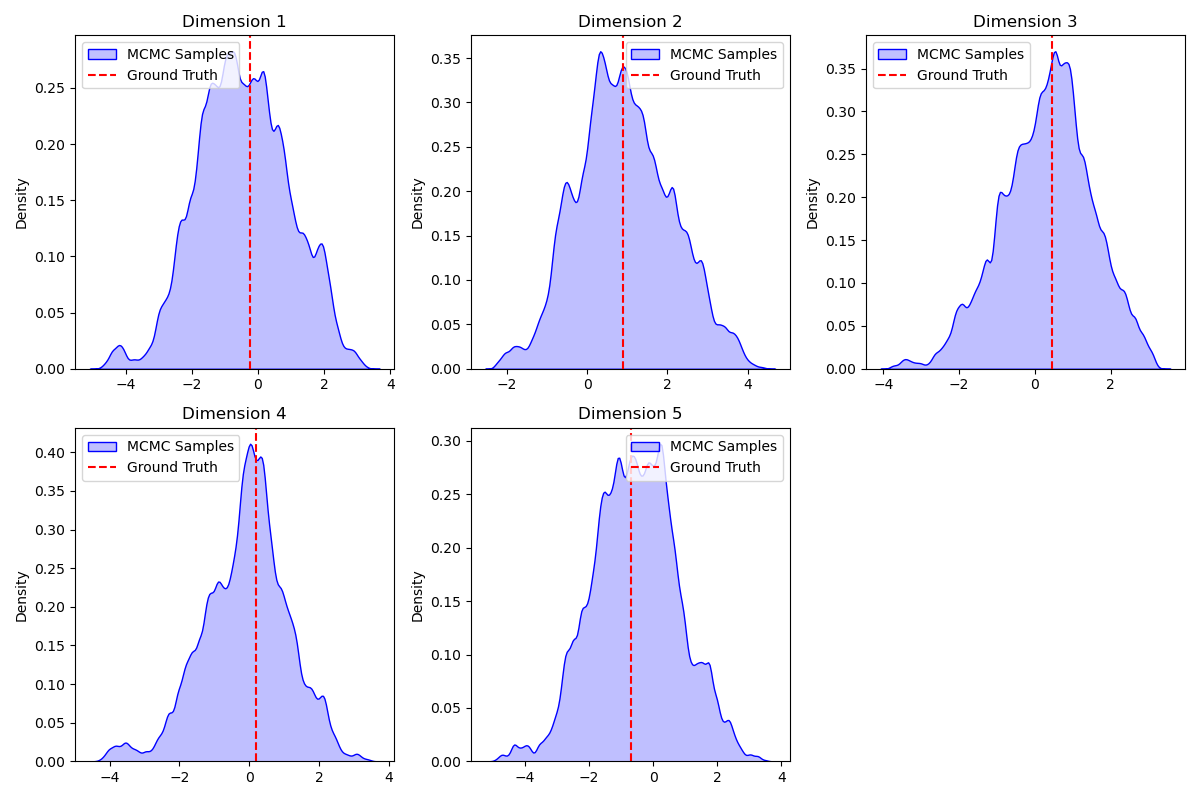
\includegraphics[width=\textwidth]{/mnt/c/workspace/study/Inverse Problem and Data Assimilation/project/Project1/pic/last_point_4000000.png} % Replace with actual image file
  \caption{First 5 Dimension Distribution (4M samples)}
      \label{fig:dim1-4m}
  \end{subfigure}
  \hfill
  \begin{subfigure}[h]{0.45\textwidth}
      \centering
      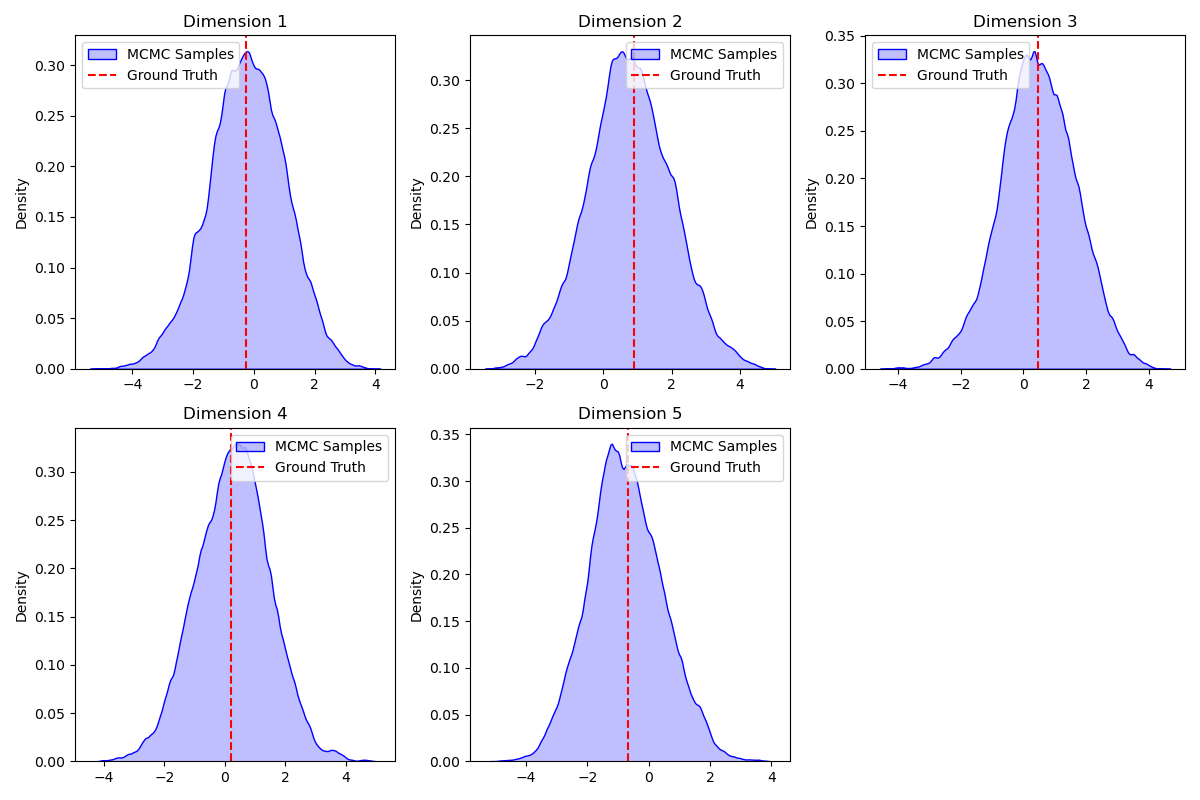
\includegraphics[width=\textwidth]{/mnt/c/workspace/study/Inverse Problem and Data Assimilation/project/Project1/pic/last_point_30000000.png} % Replace with actual image file
  \caption{First 5 Dimension Distribution (30M samples)}
      \label{fig:dim1-30m}
  \end{subfigure}

  \caption{Full observations result(part1)}
  \label{fig:distribution-comparison1}
\end{figure}
\begin{figure}[H] % Floating environment (ensure subcaptions are inside this)
  % Second Row
  \begin{subfigure}[h]{0.4\textwidth}
      \centering
      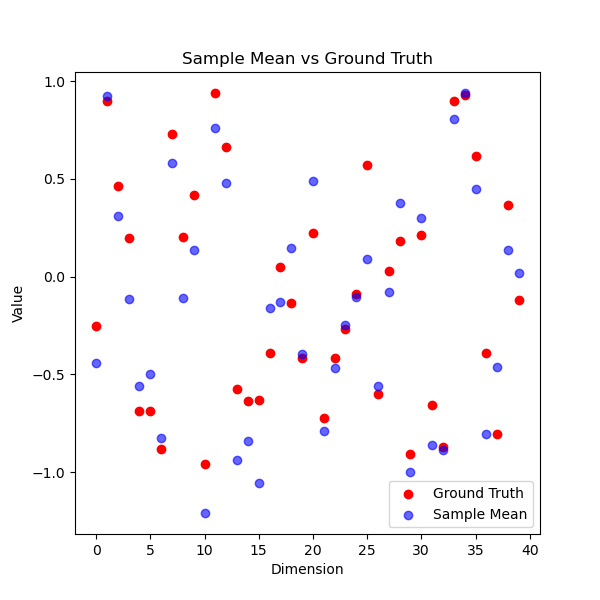
\includegraphics[width=\textwidth]{/mnt/c/workspace/study/Inverse Problem and Data Assimilation/project/Project1/pic/last_point_4000000_2.png} % Replace with actual image file
  \caption{Comparison of All Dimensions (4M samples)}
      \label{fig:comparison-4m}
  \end{subfigure}
  \hfill
  \begin{subfigure}[h]{0.4\textwidth}
      \centering
      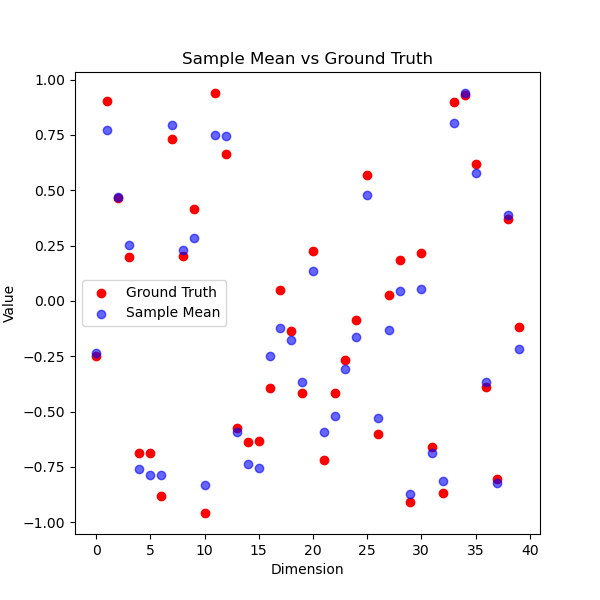
\includegraphics[width=\textwidth]{/mnt/c/workspace/study/Inverse Problem and Data Assimilation/project/Project1/pic/last_point_30000000_2.png} % Replace with actual image file
  \caption{Comparison of All Dimensions (30M samples)}
      \label{fig:comparison-30m}
  \end{subfigure}

  \caption{Full observations result(part2)}
  \label{fig:distribution-comparison2}
\end{figure}

When using partial observations, the error does not seem to converge as the number of samples increases.
\begin{table}[H]
  \begin{tabular}{|l|l|l|l|}
  \hline
  num-samples & 150000             & 300000    & 3000000        \\ \hline
  SSE         & 172.800723 & 309.825094 & 4340.741020 \\ \hline
  \end{tabular}
\end{table}

I tried some observations in 38 or 39 dimensions and found that it seems that only the unobserved dimensions and nearby dimensions will produce huge errors, while most other dimensions are relatively accurate. For details, see the following two comparison charts of the sampling mean and true value of each dimension.
\begin{figure}[H]
\begin{subfigure}[h]{0.45\textwidth}
  \centering
  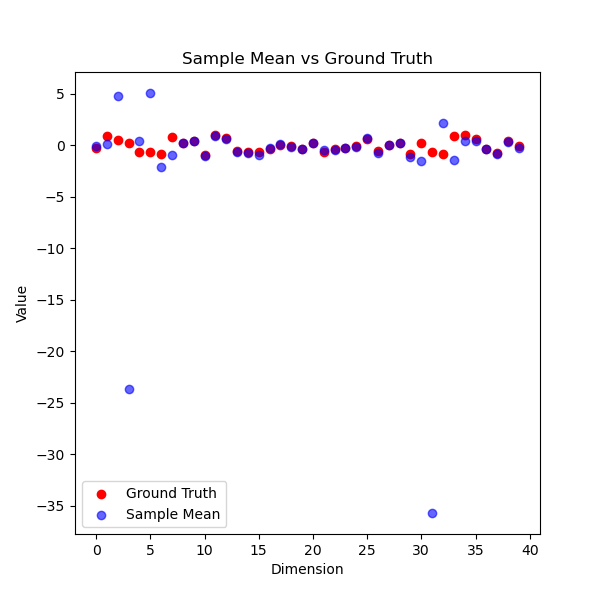
\includegraphics[width=\textwidth]{/mnt/c/workspace/study/Inverse Problem and Data Assimilation/project/Project1/pic/dim38_2.png} % Replace with actual image file
 \caption{Sampling Mean vs. True Value (38 Dimensions)}
  \label{fig:mean-vs-true-38d}
\end{subfigure}
\hfill
\begin{subfigure}[h]{0.45\textwidth}
  \centering
  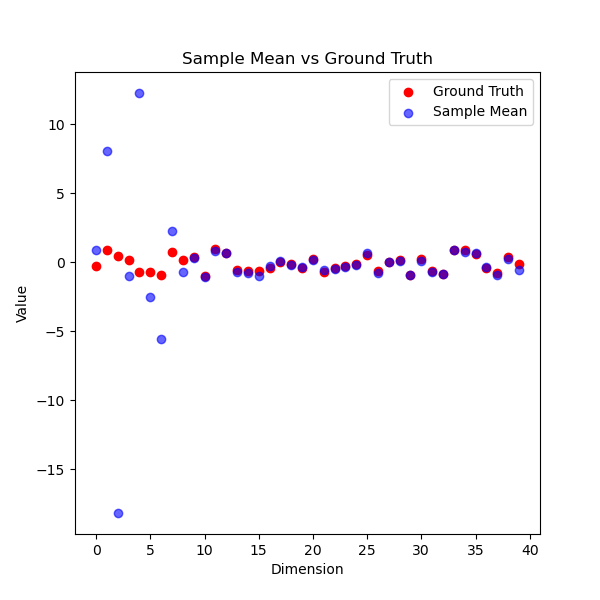
\includegraphics[width=\textwidth]{/mnt/c/workspace/study/Inverse Problem and Data Assimilation/project/Project1/pic/dim39_20000000_2.png} % Replace with actual image file
  \caption{Sampling Mean vs. True Value (39 Dimensions)}
  \label{fig:mean-vs-true-39d}
\end{subfigure}
\caption{Parital observations result}
\label{fig:part_obs_distribution-comparison}
\end{figure}

\section{Repeat the same with the ML Lorenz96 model}

The script \verb|mcmc_ml.py| has completed the task.

\begin{table}[H]
  \begin{tabular}{|l|l|l|l|l|l|}
  \hline
  num-samples & 20000            & 40000            & 80000             & 150000             & 3000000            \\ \hline
  SSE         & 26.808195 & 39.710715 & 44.904860 & 26.932605 & 5.450223 \\ \hline
  \end{tabular}
\end{table}

As can be seen from the table, although the average error of the MCMC sampling performed using the ML model is also converging, the accuracy is not high. More sampling times are required to achieve the same error accuracy. And the running speed is also slower.

The number of iterations of the drawn image is less than that in the previous section because the running time is too long.
\begin{figure}[H] % Floating environment (ensure subcaptions are inside this)
  \centering
  % First Row
  \begin{subfigure}[h]{0.45\textwidth}
      \centering
      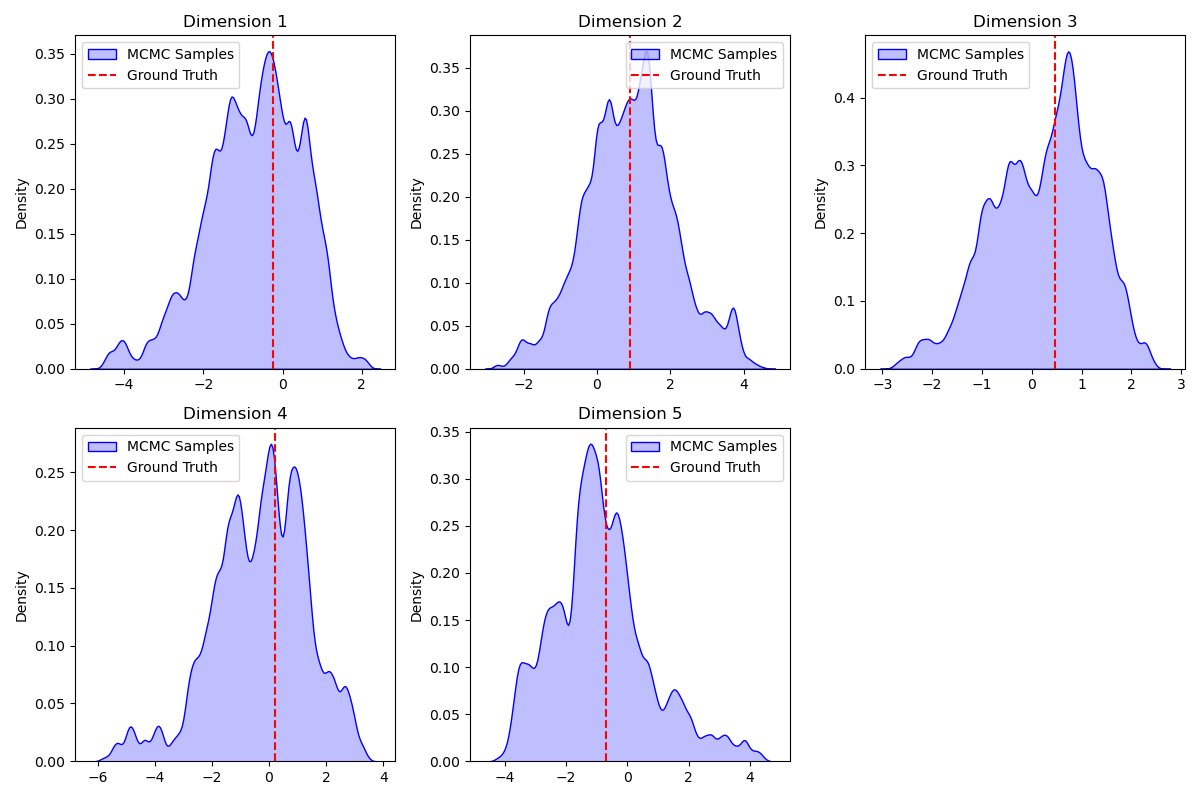
\includegraphics[width=\textwidth]{/mnt/c/workspace/study/Inverse Problem and Data Assimilation/project/Project1/pic/last_point_ml2000000.png} % Replace with actual image file
  \caption{First 5 Dimension Distribution (2M samples)}
      \label{fig:dim1-2m}
  \end{subfigure}
  \hfill
  \begin{subfigure}[h]{0.45\textwidth}
      \centering
      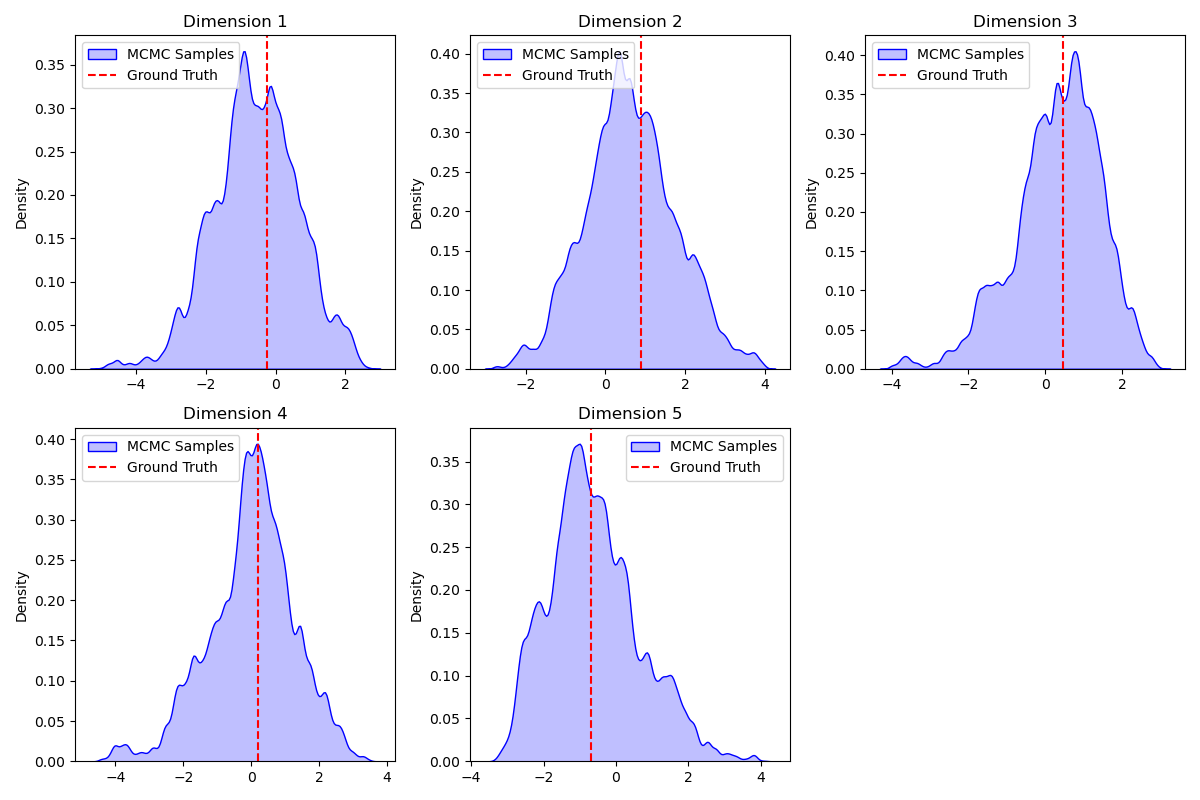
\includegraphics[width=\textwidth]{/mnt/c/workspace/study/Inverse Problem and Data Assimilation/project/Project1/pic/last_point_ml3000000.png} % Replace with actual image file
  \caption{First 5 Dimension Distribution (3M samples)}
      \label{fig:dim1-3m}
  \end{subfigure}

  \begin{subfigure}[h]{0.4\textwidth}
      \centering
      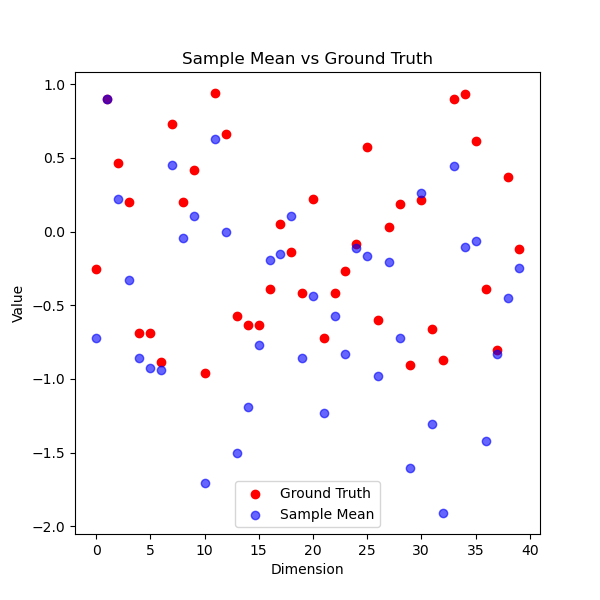
\includegraphics[width=\textwidth]{/mnt/c/workspace/study/Inverse Problem and Data Assimilation/project/Project1/pic/last_point_ml2000000_2.png} % Replace with actual image file
  \caption{Comparison of All Dimensions (2M samples)}
      \label{fig:comparison-2m}
  \end{subfigure}
  \hfill
  \begin{subfigure}[h]{0.4\textwidth}
      \centering
      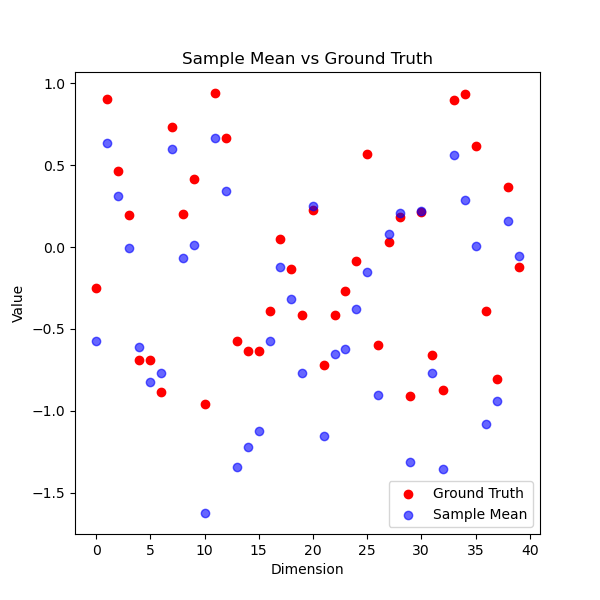
\includegraphics[width=\textwidth]{/mnt/c/workspace/study/Inverse Problem and Data Assimilation/project/Project1/pic/last_point_ml3000000_2.png} % Replace with actual image file
  \caption{Comparison of All Dimensions (3M samples)}
      \label{fig:comparison-3m}
  \end{subfigure}

  \caption{Full observations result of ML model MCMC}
  \label{fig:distribution-comparison_ml}
\end{figure}

I also tried using mcmc of the ml model for partial observations and the results also seemed to not converge.
\begin{table}[H]
  \begin{tabular}{|l|l|l|l|}
  \hline
  num-samples & 150000            & 300000            & 3000000            \\ \hline
  SSE         & 172.800723 & 309.825094 & 4340.741020\\ \hline
  \end{tabular}
\end{table}

\section{Solve the inverse problem of Darcy equation}

The script \verb|mcmc_dancy.py| has completed the task.

I found that the required true value at each point is often only 0 or 1, so I tried to perform mcmc sampling only in the value range of 0 and 1, and the effect did become better.

\begin{table}[H]
  \begin{tabular}{|l|l|l|l|l|l|l|}
  \hline
  num-samples & 100            & 1000            & 10000       & 100000 & 1000000    \\ \hline
  SSE         & 321.9372 & 280.0072 & 229.1814 & 186.9065 & 181.1333\\ \hline
  SSE(01 range sample)         &  &  & 189.1669 & 146.8316 & 143.3735\\ \hline
  \end{tabular}
  \caption{SSE Trends(in 32*32 grid)}
\end{table}
The following figures illustrate the comparison results for different sampling strategies and sampling counts:

1. \textbf{Comparison of Two Sampling Strategies}:
   Figure~\ref{fig:comparison-16x16} shows the results of two different sampling strategies for a 16*16 resolution with \texttt{num\_samples} = 6,000,000. The results indicate that sampling within the 01 range improves performance.

2. \textbf{Effect of Sampling Count at 32*32 Resolution}:
   Figures~\ref{fig:comparison-32x32} demonstrate the results for a 32*32 resolution with the 01 range sampling strategy. Different numbers of samples (\texttt{num\_samples} = 10,000, 100,000, and 1,000,000) were used. The results show that increasing the number of samples leads to improved outcomes.

\begin{figure}[htbp]
    \centering
    % Row 1: Comparison of Two Sampling Strategies (16x16 Resolution)
    \begin{subfigure}[t]{0.45\textwidth}
        \centering
        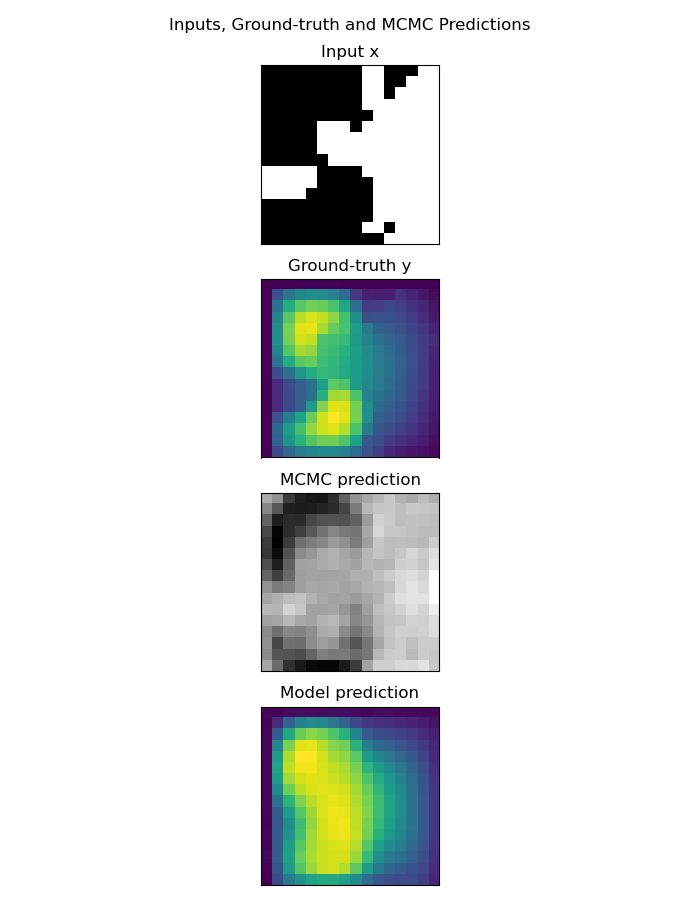
\includegraphics[width=\textwidth]{/mnt/c/workspace/study/Inverse Problem and Data Assimilation/project/Project1/pic/16*16_6000000.png} % Replace with actual image file
        \caption{16*16 Resolution with Sampling Strategy A (\texttt{num\_samples} = 6,000,000).}
        \label{fig:16x16-strategy-a}
    \end{subfigure}
    \hfill
    \begin{subfigure}[t]{0.45\textwidth}
        \centering
        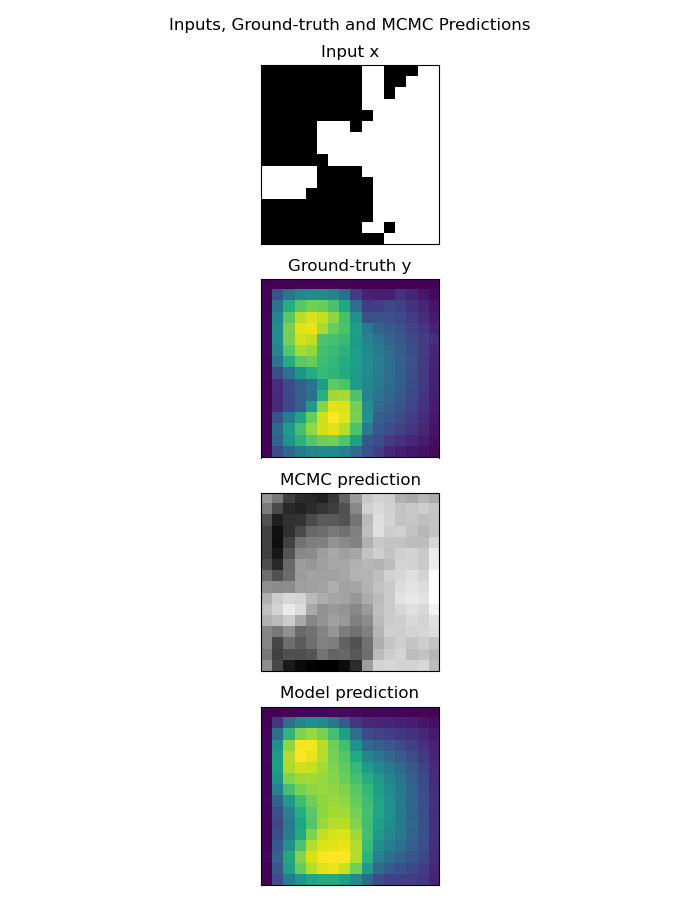
\includegraphics[width=\textwidth]{/mnt/c/workspace/study/Inverse Problem and Data Assimilation/project/Project1/pic/16*16_6000000_01.png} % Replace with actual image file
        \caption{16×16 Resolution with Sampling Strategy B (\texttt{num\_samples} = 6,000,000).}
        \label{fig:16x16-strategy-b}
    \end{subfigure}
    \caption{Comparison of Two Sampling Strategies at 16*16 Resolution.}
    \label{fig:comparison-16x16}

  \end{figure}
  \begin{figure}[htbp]
    % Row 2: Effect of Sampling Count (32x32 Resolution)
    \vspace{0.5cm} % Add some vertical space between rows
    \begin{subfigure}[t]{0.33\textwidth}
        \centering
        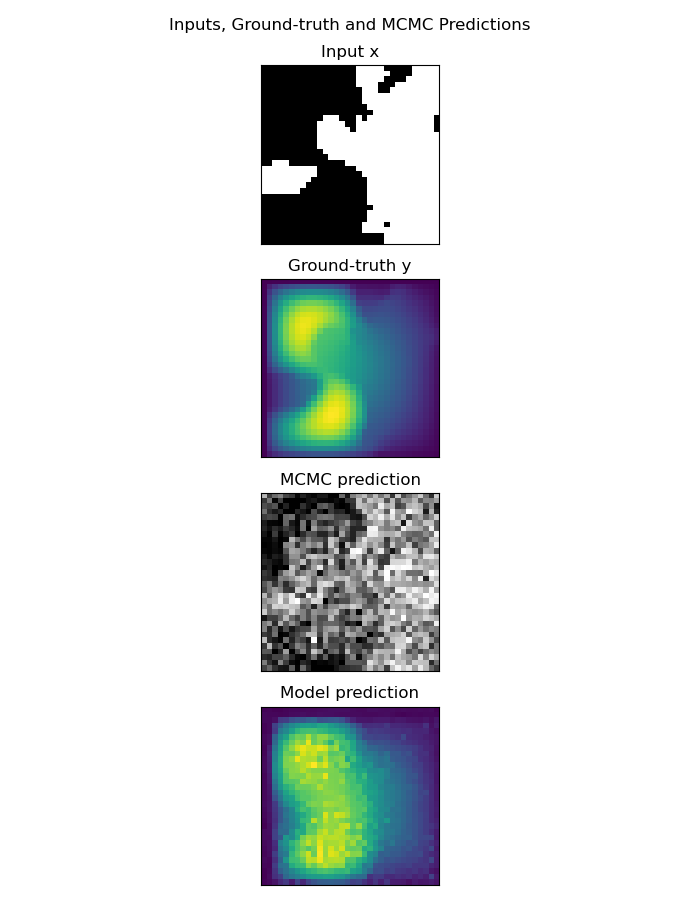
\includegraphics[width=\textwidth]{/mnt/c/workspace/study/Inverse Problem and Data Assimilation/project/Project1/pic/32*32_10000_01_0.01.png} % Replace with actual image file
        \caption{\texttt{num\_samples} = 10,000.}
        \label{fig:32x32-10k}
    \end{subfigure}
    \hfill
    \begin{subfigure}[t]{0.32\textwidth}
        \centering
        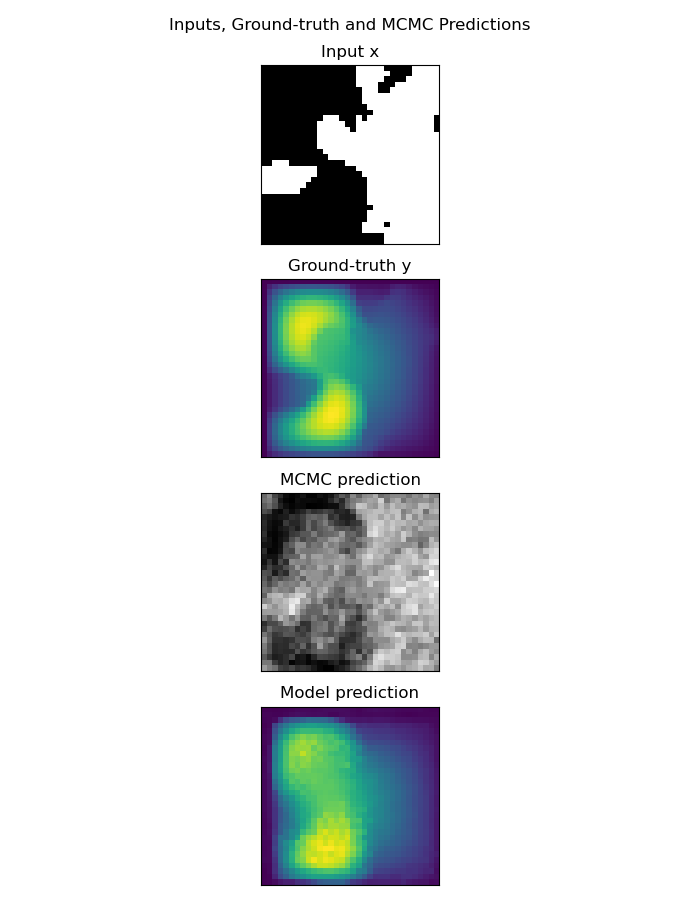
\includegraphics[width=\textwidth]{/mnt/c/workspace/study/Inverse Problem and Data Assimilation/project/Project1/pic/32*32_100000_01_0.01.png} % Replace with actual image file
        \caption{\texttt{num\_samples} = 100,000.}
        \label{fig:32x32-100k}
    \end{subfigure}
    \hfill
    \begin{subfigure}[t]{0.33\textwidth}
        \centering
        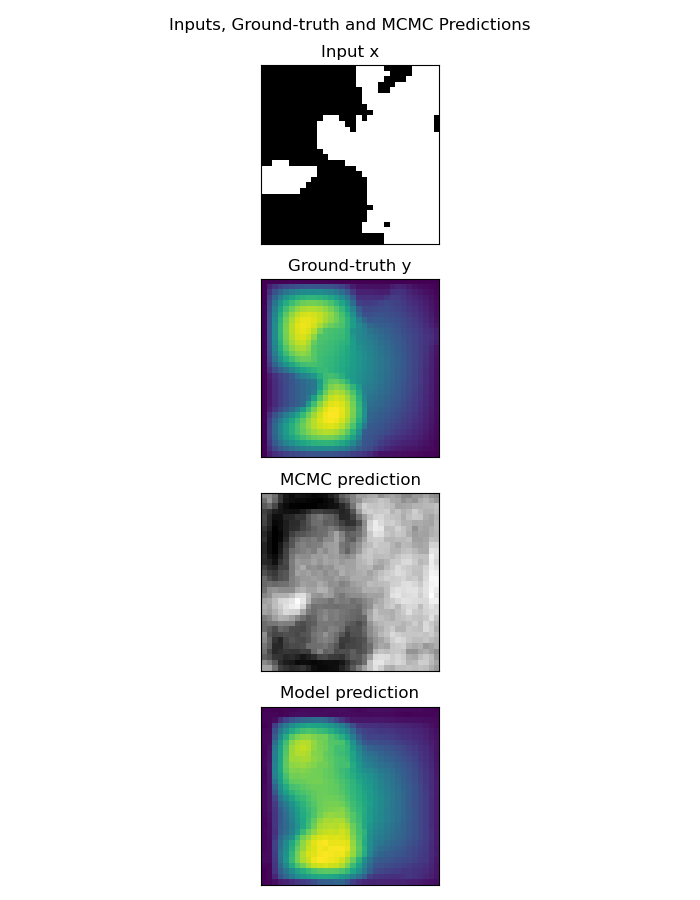
\includegraphics[width=\textwidth]{/mnt/c/workspace/study/Inverse Problem and Data Assimilation/project/Project1/pic/32*32_1000000_01_0.01.png} % Replace with actual image file
        \caption{\texttt{num\_samples} = 1,000,000.}
        \label{fig:32x32-1m}
    \end{subfigure}
    \caption{Effect of Sampling Count at 32*32 Resolution with the 01 Range Sampling Strategy.}
    \label{fig:comparison-32x32}
\end{figure}
\end{document}